\documentclass[12pt]{article}
\usepackage[left=1in,top=1in,right=1in,bottom=1in]{geometry}
\usepackage[font=footnotesize]{caption}
\usepackage{parskip}
\usepackage{times}
\usepackage{graphicx}
\usepackage{mathtools}
\usepackage{gensymb}
\usepackage{placeins}
\usepackage{graphicx}
\usepackage{enumitem}
\usepackage{verbatim}	% code text
\usepackage{siunitx}	% math units
\usepackage{hyperref}	% include urls

\setlength{\parskip}{\baselineskip}
\setlist[itemize]{noitemsep}
\setlist[enumerate]{noitemsep}

\begin{document}

	\section{Coordinate System}
	
	We usually represent the angular orientation of an aircraft using Tait-Bryan Angles following \\
	$z$-$y'$-$x''$ (intrinsic rotations) convention, also known as nautical angles, 
	also known as heading, elevation and bank, also known as yaw, pitch and roll. 
	The latter three terms are also used for the three aircraft principal axes.
	
	Some terminology:
	\begin{itemize}
		\item Let $x_b$ be the longitudinal axis (roll), out the nose of the plane.
		\item Let $y_b$ be the lateral axis (pitch), out the right wing.
		\item Let $z_b$ be the vertical axis (yaw), pointing out the bottom of the plane.
	\end{itemize}
	
	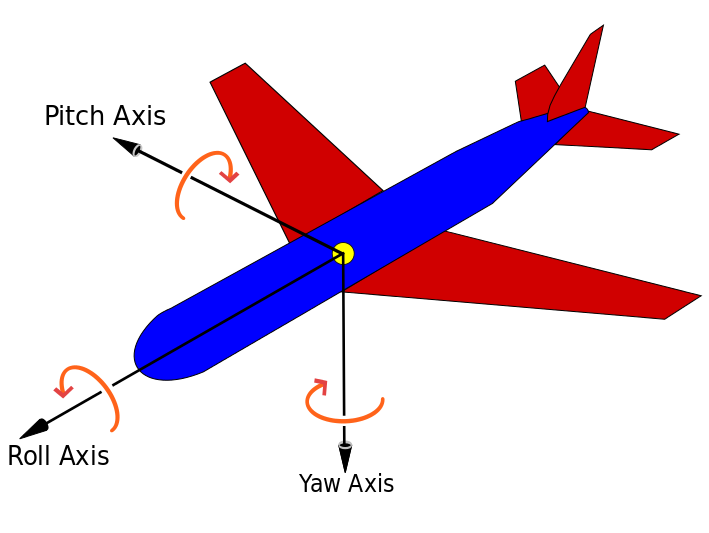
\includegraphics[width=4in]{aircraft_axes.png}
	
	By default, this coordinate system is aligned with the Earth frame:
	\begin{itemize}
		\item $x_b = x_E$ - positive in the direction of north
		\item $y_b = y_E$ - positive in the direction of east
		\item $z_b = z_E$ - positive towards the center of the Earth
	\end{itemize}
	
	To define an arbitrary angular orientation, we follow this procedure:
	\begin{enumerate}
		\item Yaw by $\psi$ about $z_b$.
		\item Pitch by $\theta$ about $y_b$.
		\item Roll by $\phi$ about $x_b$.
	\end{enumerate}
	Note that the body frame rotates with the aircraft as we go through the procedure. 
	Note also that right hand rule convention is always followed. 
	
	\section{Controller}
	
	We want to control the pitch and roll of the aircraft. 
	(We've given up on yaw because using gravity with the Launchpad only gives us about two detectable axes of rotation.)
	
	More specifically, we want to map the angular orientation of the joystick to an angular velocity about a pitch or roll axis. 
	Let $\vec{g}_c$ be the acceleration of gravity in the coordinate system of the control column.
	Then define the following functions:
	\begin{itemize}
		\item $\text{pitcher} : \vec{g}_c \mapsto \dot{\theta}$
		\item $\text{roller} : \vec{g}_c \mapsto \dot{\phi}$
	\end{itemize} 
	
	If we wanted to be more accurate, the controller would not modify the angular velocity of the aircraft directly, 
	but rather adjust the position of simulated elevators and ailerons. 
	This would ensure that the aircraft is reliably uncontrollable if we stalled it or whatever.
	
	If the controller is too aggresive, it could flip the aircraft 180 degrees away from its velocity and it would be flying backwards, which isn't very realistic. 
	(Hopefully the simulated flight dynamics stuffs would provide a resistive force to prevent this sort of thing from happening. 
	If so, then controlling the angular velocity might be not too inaccurate.) But for now, we'll assume that the controller directly controls angular velocity of the aircraft, because it's simpler that way.
	
	\section{First Method: Simple projection}
	
	We want the orientation of the controller to mirror the direction of the change in angular velocity of the aircraft. 
	i.e., if we pitch the controller forwards, we expect the aircraft to do the same. 
	
	We will define three mutually orthogonal axes in the reference frame of the controller with the following unit vectors:
	\begin{itemize}
		\item $\vec{s}$ (\verb|STICK|) : The direction of the grippy part of the joystick if this were a normal joystick. Points away from the centre of the earth when controller is in rest state.
		\item $\vec{p}$ (\verb|PITCH_AXIS|) : The rotation axis for pitch. Points right when controller is in rest state.
		\item $\vec{r}$ (\verb|ROLL_AXIS|) : The rotation axis for roll. Points forward when controller is in rest state.
	\end{itemize}
	For convenience, we will also define the following two unit vectors:
	\begin{itemize}
		\item $\vec{p}_\perp$ (\verb|PITCH_PERP|) : The vector obtained by rotating $\vec{s}$ 90 degrees CCW about $\vec{p}$.
		\item $\vec{r}_\perp$ (\verb|ROLL_PERP|) :  The vector obtained by rotating $\vec{s}$ 90 degrees CCW about $\vec{r}$.
	\end{itemize}
	
	The Launchpad will detect an acceleration vector $\vec{g}$ that is pointing out from the centre of the Earth. 
	Assuming that other accelerations such as those from moving the controller are negligible, we now have a vertical reference. 
	
	Assume the following:
	\begin{itemize}
		\item If $\vec{g} \parallel \verb|STICK|$, then $\dot{\theta} = \dot{\phi} = \SI{0}{\radian\per\second}$
		\item For pitching, consider only the projection of $\vec{g}$ in the $\langle \vec{s}, \vec{p}_\perp \rangle$-plane.
		\item For rolling, consider only the projection of $\vec{g}$ in the $\langle \vec{s}, \vec{r}_\perp \rangle$-plane.
	\end{itemize}
	Let $k_1$ be a scaling factor for pitch and $k_2$ be a scaling factor for roll, both in radians per second per radian. Then:
		$$\dot{\theta} = -k_1\;\text{atan2}(\vec{g} \cdot \vec{p}_\perp, \vec{g} \cdot \vec{s})$$
		$$\dot{\phi} = -k_2\;\text{atan2}(\vec{g} \cdot \vec{r}_\perp, \vec{g} \cdot \vec{s})$$
	To establish a maximum rate, we can replace the output of $\text{atan2}$ with a specified max angle if the value is exceeded.
	
	\subsection{Issues}
	
	Consider the case where we roll the controller left more than 90$\si{\degree}$. 
	The above formulas will suddenly output maximum pitch, which is not good.
		
	
	
	
	\section{References}

	\urlstyle{same}
	
	\begin{itemize}
		\item Tait-Bryan angles: \url{https://en.wikipedia.org/wiki/Euler_angles#Tait.E2.80.93Bryan_angles}	
		\item Degrees of freedom (mechanics): \url{https://en.wikipedia.org/wiki/Degrees_of_freedom_(mechanics)}
	\end{itemize}

\end{document}